\begin{center}
  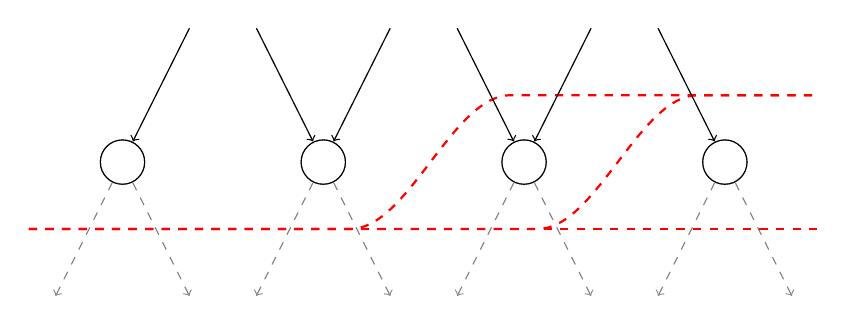
\begin{tikzpicture}[scale=1.7, every node/.style={transform shape}]
    % cut coordinates
    \coordinate (cut_start) at (-0.7,-0.5);
    \coordinate (cut_end_low) at (5.2,-0.5);
    \path (cut_end_low) +(0,1) coordinate (cut_end_high);

    % --------------------------------------------------------------------------
    % before
    \onslide<1> {
      \node[shape = circle, draw = gray] at (0,0)  (0_before) {};
      \draw[gray, dashed, <-] (0_before) -- ++(0.5,1.0);
    }

    % after
    \onslide<2-> {
      \node[shape = circle, draw = black] at (0,0) (0_after) {};
      \draw[black, <-] (0_after) -- ++(0.5,1.0);

      \draw[gray, dashed, ->] (0_after) -- ++(-0.5,-1);
      \draw[gray, dashed, ->] (0_after) -- ++(0.5,-1);
    }

    % --------------------------------------------------------------------------
    % before
    \onslide<-2> {     
      \node[shape = circle, draw = gray] at (1.5,0) (1_before) {};
      \draw[gray, dashed, <-] (1_before) -- ++(-0.5,1.0);
      \draw[gray, dashed, <-] (1_before) -- ++(0.5, 1.0);
    }

    % after
    \onslide<3-> {
      \node[shape = circle, draw = black] at (1.5,0) (1_after) {};
      \draw[black, <-] (1_after) -- ++(-0.5,1.0);
      \draw[black, <-] (1_after) -- ++(0.5, 1.0);

      \draw[gray, dashed, ->] (1_after) -- ++(-0.5,-1);
      \draw[gray, dashed, ->] (1_after) -- ++(0.5,-1);
    }

    % cut
    \onslide<4> {
      \draw[thick, dashed, red]
        (cut_start) -- ++(2.4,0.0) cos ++(0.6,0.5) sin ++(0.6,0.5) -- (cut_end_high)
      ;
    }
    
    % --------------------------------------------------------------------------
    % before
    \onslide<-4> {
      \node[shape = circle, draw = gray] at (3.0,0) (2_before) {};
      \draw[gray, dashed, <-] (2_before) -- ++(-0.5,1.0);
      \draw[gray, dashed, <-] (2_before) -- ++(0.5,1.0);
    }

    % after    
    \onslide<5-> {
      \node[shape = circle, draw = black] at (3.0,0) (2_after) {};
      \draw[black, <-] (2_after) -- ++(-0.5, 1.0);
      \draw[black, <-] (2_after) -- ++(0.5, 1.0);

      \draw[gray, dashed, ->] (2_after) -- ++(-0.5,-1);
      \draw[gray, dashed, ->] (2_after) -- ++(0.5,-1);
    }

    % cut
    \onslide<5> {
      \draw[thick, dashed, red]
        (cut_start) -- ++(3.8,0.0) cos ++(0.6,0.5) sin ++(0.6,0.5) -- (cut_end_high)
      ;
    }

    % --------------------------------------------------------------------------
    % before
    \onslide<-5> {
      \node[shape = circle, draw = gray] at (4.5,0) (3_before) {};
      \draw[gray, dashed, <-] (3_before) -- ++(-0.5,1.0);
    }

    % after
    \onslide<6-> {
      \node[shape = circle, draw = black] at (4.5,0) (3_after) {};
      \draw[black, <-] (3_after) -- ++(-0.5,1.0);      

      \draw[gray, dashed, ->] (3_after) -- ++(-0.5,-1);
      \draw[gray, dashed, ->] (3_after) -- ++(0.5,-1);
    }

    % cut
    \onslide<6> {
      \draw[thick, dashed, red]
        (cut_start) -- (cut_end_low)
      ;
    }
  \end{tikzpicture}
\end{center}